%%%%%%%%%%%%%%%%%%%%%%%%%%%%%%%%%%%%%%%%%%%%%%%%%%%%%%%%%%%%%%%%%%%%%%%%%%%%%%%%
% DOCUMENT SPECIFICATION
%%%%%%%%%%%%%%%%%%%%%%%%%%%%%%%%%%%%%%%%%%%%%%%%%%%%%%%%%%%%%%%%%%%%%%%%%%%%%%%%
% \documentclass[twoside,a4paper]{scrartcl}        % Koma-script class
\documentclass[a4paper]{scrartcl}               % Koma-script class

%----------------------------------------------------------------------------------------
% PREAMBLE: PACKAGES AND CONFIGURATIONS
%----------------------------------------------------------------------------------------
% !TEX root = main.tex
%
% TODO: Have a clearer separation between ZHAW Thesis class and this preamble.

%%%%%%%%%%%%%%%%%%%%%%%%%%%%%%%%%%%%%%%%%%%%%%%%%%%%%%%%%%%%%%%%%%%%%%%%%%%%%%%%
% Fonts and characters
%%%%%%%%%%%%%%%%%%%%%%%%%%%%%%%%%%%%%%%%%%%%%%%%%%%%%%%%%%%%%%%%%%%%%%%%%%%%%%%%

% Support for special characters
\usepackage[utf8]{inputenc}    % Input encoding: Support non-ascii characters
\usepackage[T1]{fontenc}       % Font encoding: T1 is good choice for Europe

% Set main fonts
% Fonts catalogue: https://tug.org/FontCatalogue/
\usepackage{mathpazo}          % Use the Palatino font by default
\usepackage{beramono}          % Override the monospace/typewriter font

\usepackage{amssymb}           % Maths
\usepackage{amsmath}           % Maths 
\usepackage{numprint}          % For nicely printing large numbers
\usepackage{lmodern}           % Use LaTeX math fonts, requires T1
\usepackage[normalem]{ulem}    % Strikethrough text.

\usepackage{pdfpages}

% ZHAW title font
% Try to load Helvetica Rounded Bold, and OpenType font.
% Loading OTF or system fonts is possible with XeLaTeX.
% If the document is compiled using pdfLaTeX, resort 
\usepackage{ifxetex}
\ifxetex
    \usepackage{fontspec}
    \newfontfamily\zhawtitlefont{Helvetica Rounded Bold}
\else
    \newcommand{\zhawtitlefont}{\scshape}
\fi

\newcommand{\boldit}[1]{\textit{\textbf{#1}}}

% Set Helvetica as the default font
\usepackage[scaled]{helvet}
\renewcommand{\familydefault}{\sfdefault}

%%%%%%%%%%%%%%%%%%%%%%%%%%%%%%%%%%%%%%%%%%%%%%%%%%%%%%%%%%%%%%%%%%%%%%%%%%%%%%%%
% Comments
%%%%%%%%%%%%%%%%%%%%%%%%%%%%%%%%%%%%%%%%%%%%%%%%%%%%%%%%%%%%%%%%%%%%%%%%%%%%%%%%

\usepackage[color=cyan,colorinlistoftodos]{todonotes}
\newcommand{\replace}[2]{{\sout{#1}} \textcolor{cyan}{#2}}
\newcommand{\note}[1]{\textcolor{cyan}{#1}}

%%%%%%%%%%%%%%%%%%%%%%%%%%%%%%%%%%%%%%%%%%%%%%%%%%%%%%%%%%%%%%%%%%%%%%%%%%%%%%%%
% Colors
%%%%%%%%%%%%%%%%%%%%%%%%%%%%%%%%%%%%%%%%%%%%%%%%%%%%%%%%%%%%%%%%%%%%%%%%%%%%%%%%

% Set up colors
\usepackage[dvipsnames]{xcolor} % Color management
% \PassOptionsToPackage{dvipsnames}{xcolor}  % Had to change this.

% ZHAW Blue: Pantone 2945 U / R0 G100 B166
\definecolor{zhawblue}{rgb}{0.00, 0.39, 0.65}
\definecolor{zhawlightblue}{rgb}{0.82, 0.88, 0.93}
% Colors related to code listings
\definecolor{codegreen}{rgb}{0,0.6,0}
\definecolor{codegray}{rgb}{0.5,0.5,0.5}
\definecolor{codepurple}{rgb}{0.58,0,0.82}
\definecolor{codebackground}{rgb}{0.93,0.94,0.95}
% Colors related to tables
\definecolor{tablegray}{rgb}{0.9,0.9,0.9}
\colorlet{tableheader}{tablegray}
% Colors related to hyperref
\definecolor{linkcolor}{rgb}{0.00, 0.39, 0.65}
\definecolor{urlcolor}{rgb}{0.00, 0.39, 0.65}

%%%%%%%%%%%%%%%%%%%%%%%%%%%%%%%%%%%%%%%%%%%%%%%%%%%%%%%%%%%%%%%%%%%%%%%%%%%%%%%%
% Environments
%%%%%%%%%%%%%%%%%%%%%%%%%%%%%%%%%%%%%%%%%%%%%%%%%%%%%%%%%%%%%%%%%%%%%%%%%%%%%%%%

% \usepackage[ngerman]{babel}    % Language support
\usepackage[english]{babel}    % Language support
\usepackage[                    % Create hypertext links
    colorlinks=true, 
    allbordercolors={white}, 
    linkcolor=linkcolor,
    citecolor=linkcolor, 
    filecolor=linkcolor,
    linktoc=all, 
    urlcolor=urlcolor
    ]{hyperref}

\usepackage{graphicx}          % Include graphics
\usepackage{float}             % Improved interface for floating objects
\usepackage{tabularx}          % Create nicer tables
\usepackage{multirow}          % Merge rows in tables
\usepackage{booktabs}          % To further beautify tables
\usepackage{longtable}         % For tables that span multiple pages
\usepackage{caption}           % Customized caption
\usepackage{subcaption}        % Subfigure captions
\usepackage{makecell}          % Per-cell formatting in tables (\makecell)
\usepackage{pdfpages}          % Required to include PDF files/graphics (\includepdf)
\usepackage{colortbl}          % Tables with colors

\usepackage{todonotes}         % Introduces the command \todo
\setlength{\marginparwidth}{2.5cm} % Adjust this if the todo notes are out of margins
\usepackage{array,ragged2e}    % For ragged alignment of multi-line table cells

% Adjust tables
\colorlet{tableheadcolor}{gray!25}                % Table header colour
\newcommand{\headcol}{\rowcolor{tableheadcolor}}% % The color of the head
\newcommand{\topline}{\arrayrulecolor{black}      %
                      \specialrule{0.1em}{\abovetopsep}{0.5pt}%
                      \arrayrulecolor{tableheadcolor}%
                      \specialrule{\belowrulesep}{0pt}{-3pt}%
            \arrayrulecolor{black}
            }
\newcommand{\midline}{\arrayrulecolor{tableheadcolor}
            \specialrule{\aboverulesep}{-1pt}{0pt}%
            \arrayrulecolor{black}\specialrule{\lightrulewidth}{0pt}{0pt}%
            \arrayrulecolor{white}\specialrule{\belowrulesep}{0pt}{-3pt}%
            \arrayrulecolor{black}
            }
\newcommand{\bottomline}{\arrayrulecolor{white}\specialrule{\aboverulesep}{0pt}{-2pt}%
            \arrayrulecolor{black}\specialrule{\heavyrulewidth}{0pt}{\belowbottomsep}}%

% Create boxes as follows:
% \begin{colorbox}{red}{2}
\usepackage{tcolorbox}
\newtcolorbox{textbox}[2]{
    arc=3pt,
    boxrule=#2pt,
    colback=#1!25!white,
    width=\textwidth,
    halign=left,
    valign=center,
    colframe=#1!75!black
}

%%%%%%%%%%%%%%%%%%%%%%%%%%%%%%%%%%%%%%%%%%%%%%%%%%%%%%%%%%%%%%%%%%%%%%%%%%%%%%%%
% Code listings
%%%%%%%%%%%%%%%%%%%%%%%%%%%%%%%%%%%%%%%%%%%%%%%%%%%%%%%%%%%%%%%%%%%%%%%%%%%%%%%%
\captionsetup{format=plain,             % plain or hang
              justification=justified,  % justified, centering, raggedright, ...
              labelfont=bf,
              font=small,
              margin=20pt}
              

%%%%%%%%%%%%%%%%%%%%%%%%%%%%%%%%%%%%%%%%%%%%%%%%%%%%%%%%%%%%%%%%%%%%%%%%%%%%%%%%
% Code listings
%%%%%%%%%%%%%%%%%%%%%%%%%%%%%%%%%%%%%%%%%%%%%%%%%%%%%%%%%%%%%%%%%%%%%%%%%%%%%%%%

\newcommand{\code}[1]{\texttt{#1}}



% Setup code listings
\usepackage{listings}
\lstdefinestyle{mystyle}{
    backgroundcolor=\color{codebackground},   
    commentstyle=\color{codegreen},
    keywordstyle=\color{magenta},
    numberstyle=\tiny\color{codegray},
    stringstyle=\color{codepurple},
    basicstyle=\ttfamily\scriptsize,
    breakatwhitespace=false,
    breaklines=true,
%    captionpos=b,
    keepspaces=true,
    numbers=left,
    numbersep=5pt,
    showspaces=false,
    showstringspaces=false,
    showtabs=false,
    tabsize=4
}
\lstset{style=mystyle}

% minted is an alternative code listing package. (See appendix A)
% For it to run successfully, ensure the following:
% - the Python package Pygments. Install with the following command:
%       python -m pip install Pygments
% - pdflatex (or xelatex) is executed with the flag --shell-escape
%   If you are using a TEX editor, you can modify the typesetting 
%   command somewhere in the settings.
%\usepackage[outputdir=build]{minted}
%\usemintedstyle{xcode}
% For fancier coloring schemes, see here:
% https://tex.stackexchange.com/questions/585582
% One could also create an own style in Pygments
% https://pygments.org/docs/styles/#creating-own-styles


%%%%%%%%%%%%%%%%%%%%%%%%%%%%%%%%%%%%%%%%%%%%%%%%%%%%%%%%%%%%%%%%%%%%%%%%%%%%%%%%
% References
%%%%%%%%%%%%%%%%%%%%%%%%%%%%%%%%%%%%%%%%%%%%%%%%%%%%%%%%%%%%%%%%%%%%%%%%%%%%%%%%

\usepackage[autostyle=true]{csquotes} 
                               % Required to generate language-dependent quotes 
                               % in the bibliography

\usepackage[
    backend=biber,             % Use biber backend (an external tool)
    sorting=nyt,               % Sort by name, year, title
    style=apa,                 % Choose here your preferred citation style
    uniquename=false,          % Avoids creating unique author lists
    uniquelist=false           % Avoids creating unique author lists
]{biblatex}

\addbibresource{SA2.bib} % The filename of the bibliography

%%%%%%%%%%%%%%%%%%%%%%%%%%%%%%%%%%%%%%%%%%%%%%%%%%%%%%%%%%%%%%%%%%%%%%%%%%%%%%%%
% MARGIN SETTINGS
%%%%%%%%%%%%%%%%%%%%%%%%%%%%%%%%%%%%%%%%%%%%%%%%%%%%%%%%%%%%%%%%%%%%%%%%%%%%%%%%
\usepackage{geometry}
\geometry{
    paper=a4paper,       % Change to letterpaper for US letter
    %inner=2.5cm,        % Inner margin
    %outer=3.8cm,        % Outer margin
    %top=1.5cm,          % Top margin
    bottom=4.cm,         % Bottom margin
    bindingoffset=.5cm,  % Binding offset
    %showframe,          % Show the type block of the page
}

% Other layout settings
\setlength\parindent{0em} % No indent
\setlength{\parskip}{1em}
%\usepackage{parskip}


\setlength{\intextsep}{30pt}   % Distance between image and text 
\usepackage{enumitem}          % Layout control for list environments (e.g, itemize)
\setlist{noitemsep}            % Suppress extra spaces between items
%\setlist{nosep}               % Suppress spaces before/after list environments


%----------------------------------------------------------------------------------------
%   PENALTIES
%----------------------------------------------------------------------------------------

\doublehyphendemerits=10000 % No consecutive line hyphens
\brokenpenalty=10000 % No broken words across columns/pages
\widowpenalty=9999 % Almost no widows at bottom of page
\clubpenalty=9999 % Almost no orphans at top of page
\interfootnotelinepenalty=9999 % Almost never break footnotes


%%%%%%%%%%%%%%%%%%%%%%%%%%%%%%%%%%%%%%%%%%%%%%%%%%%%%%%%%%%%%%%%%%%%%%%%%%%%%%%%
% MANAGE AUTHOR LISTS
%%%%%%%%%%%%%%%%%%%%%%%%%%%%%%%%%%%%%%%%%%%%%%%%%%%%%%%%%%%%%%%%%%%%%%%%%%%%%%%%

\usepackage[affilmode=count]{authors}


% Trick: Convert the setter into a getter.
\NewDocumentCommand{\projecttitle}{m}{\renewcommand{\projecttitle}{#1}}
\NewDocumentCommand{\projecttype}{m}{\renewcommand{\projecttype}{#1}}
\NewDocumentCommand{\projectcode}{m}{\renewcommand{\projectcode}{#1}}
\NewDocumentCommand{\projectdate}{m}{\renewcommand{\projectdate}{#1}}
\NewDocumentCommand{\keywords}{m}{\renewcommand{\keywords}{#1}}

\NewDocumentCommand{\university}{m}{\renewcommand{\university}{#1}}
\NewDocumentCommand{\department}{m}{\renewcommand{\department}{#1}}
\NewDocumentCommand{\institute}{m}{\renewcommand{\institute}{#1}}
\NewDocumentCommand{\group}{m}{\renewcommand{\group}{#1}}


%----------------------------------------------------------------------------------------
%   HEADERS AND FOOTERS
%----------------------------------------------------------------------------------------

% Notes:
% - In twoside mode, left and right side pages may differ
% - Pages: left = even, right = odd
%   Chapters usually are forced to start at odd pages.
% - \markboth{left}{right} how left and right pages are marked
% - \automark is a convenience command from the scrlayer-scrpage package. It issues 
%   that \markboth is called for every \chapter and \section command.
% - Historical note: scrlayer-scrpage is the successor of scrpage2
% - Refs:
%    \markboth:  https://tex.stackexchange.com/questions/198676
%    \automark:  https://tex.stackexchange.com/questions/34269/
%    \automark*: https://tex.stackexchange.com/questions/348550/
%
\usepackage[markcase=used]{scrlayer-scrpage}
\ifoot{}% Empty inner footer by default
\ofoot{}% Empty outer footer by default
\providepairofpagestyles{basicStyle}{
    % Header specs for style basicStyle
    \clearpairofpagestyles%
    % \automark[section]{section}
    % \ihead{\headmark}% Inner header
    % \ohead[\pagemark]{\pagemark}% Outer header
    \cfoot[\pagemark]{\pagemark}% Footer with pagemark in the middle
}
\pagestyle{basicStyle}

\providepairofpagestyles[basicStyle]{reportStyle}{%
    \automark*[subsection]{}% Override right marks with section title once one is set
                         % Otherwise, use the chapter title -> basicStyle
}
% \pagestyle{reportStyle}

\KOMAoption{headsepline}{false} % set true to get a line below the header








% Includes for blind texts...
\usepackage{blindtext}
\usepackage{kantlipsum}

%----------------------------------------------------------------------------------------
% PROJECT INFORMATION: MODIFY THIS SECTION!
%----------------------------------------------------------------------------------------
\projecttitle{Deep Learning for Pixel-Level Classification of Impervious and Pervious Surfaces in Remote Sensing}
\projecttype{Term Paper 2}
\projectcode{}
\projectdate{\today}
\keywords{
    classification, 
    deep learning, 
    machine learning, 
    remote sensing, 
    land cover classification, 
    impervious surfaces, 
    pervious surfaces, 
    surface sealing, 
    urbanization, 
    environmental monitoring, 
    pixel-based analysis
}

%----------------------------------------------------------------------------------------
% AUTHORS AND AFFILIATIONS
%----------------------------------------------------------------------------------------
\addauthor{A}{Julian}{Kraft}{kraftjul@students.zhaw.ch}{1}

\addcollaborator{A}{Dr. Johann}{Junghardt}{johann.junghardt@zhaw.ch}{1}

\addaffiliation{1}
{Institute of Natural Resource Sciences}
{https://www.zhaw.ch/en/lsfm/institutes-centres/iunr/}
{Grüentalstrasse 14, Wädenswil, Switzerland}

\university{Zurich University of Applied Sciences}
\department{Life Sciences and Facility Management}
\institute{Institute of Natural Resource Sciences} 
\group{} 

\AtBeginDocument{
\hypersetup{pdftitle=\projecttitle} % Set the PDF's title to your title
\hypersetup{pdfauthor=\printauthors} % Set the PDF's author to your name
\hypersetup{pdfkeywords=\keywords} % Set the PDF's keywords to your keywords
}

\begin{document}
\hypersetup{linkcolor=black, urlcolor=black} % Make links black for first part
%----------------------------------------------------------------------------------------
% TITLE PAGE AND IMPRINT
%----------------------------------------------------------------------------------------
% !TEX root = ../main.tex

%%%%%%%%%%%%%%%%%%%%%%%%%%%%%%%%%%%%%%%%%%%%%%%%%%%%%%%%%%%%%%%%%%%%%%%%%%%%%%%%
% TITLE PAGE
%%%%%%%%%%%%%%%%%%%%%%%%%%%%%%%%%%%%%%%%%%%%%%%%%%%%%%%%%%%%%%%%%%%%%%%%%%%%%%%%

% New command to make the lines in the title page
\newcommand{\HRule}{\rule{.9\linewidth}{.6pt}} 

\newgeometry{margin=1in}
\begin{titlepage}

% Make the title page mostly inert to the parskip-setting.
\setlength{\parskip}{0pt}

\begin{center}

\includegraphics[width=0.15\textwidth]{Figures/zhaw_rgb}

\ifxetex
    \vspace{0.6cm}
    {\zhawtitlefont\color{zhawblue}\LARGE\university\par}   % University
    \vspace{0.2cm}
\else
    \vspace{0.87cm}
    {
\includegraphics[height=17.9pt]{figures/zhaw_font_eng_font}\par}
    \vspace{0.05cm}
\fi
{\Large \ifdefempty{\department}{}{Department \department\par}} % Department
\vspace{0.2cm}
{\Large \institute\par}                                     % Institute
\vspace{3.5cm}                            
\textsc{\Large \projecttype}                                % Project type
\vspace{0.2cm}
\HRule 
\vspace{0.4cm}
{\huge \bfseries \projecttitle\par}                         % Project title
\vspace{0.4cm}  
\HRule
\vspace{1cm}
                     
\textsc{\Large \projectdate}                                % Project type
\vspace{1.5cm}



\begin{footnotesize}
\begin{tabular}{lr}

% Authors
\begin{minipage}[t]{0.41\textwidth}
\begin{flushleft}
    \boldit{Author:}\\
    \printauthors[\\][email3]% No whitespace!
    \vspace{1cm}
\end{flushleft}
\end{minipage}

&

% Collaborators
\begin{minipage}[t]{0.41\textwidth}
\begin{flushright}
    \boldit{Tutor:} \\
    \printcollaborators[\\][email3]% No whitespace!
    \vspace{1cm}
\end{flushright}
\end{minipage}

\\

% Affiliations
\begin{minipage}[t]{0.41\textwidth}
\begin{flushleft}
    \boldit{Affiliations:} \\
    \printaffiliations[\\]
\end{flushleft}
\end{minipage}

&

% Industrial partners
% \begin{minipage}[t]{0.41\textwidth}
% \begin{flushright}
%     \boldit{Industry partner:} \\
%     \printcompanies[\\]
% \end{flushright}
% \end{minipage}

\end{tabular}
\end{footnotesize}

% \begin{footnotesize}
% \begin{minipage}[t]{0.4\textwidth}
% \begin{flushleft}
%     \emph{Authors:}\\
%     \printauthors[\\][compact]\\
%     \vspace{0.5cm}
%     \emph{Affiliations:} \\
%     \printaffiliations[\\]
% \end{flushleft}
% \end{minipage}
% \begin{minipage}[t]{0.4\textwidth}
% \begin{flushright}
%     \emph{Partners:} \\
%     \printcollaborators[\\][compact]\\
%     \vspace{0.5cm}
%     \emph{Industrial partner:} \\
%     \printcompanies[\\]
% \end{flushright}
% \end{minipage}
% \end{footnotesize}

\vspace{2cm}
 
\vfill

% {\large
% \projectdate\\
% \vspace{1.5cm}
% Project Code:\\
% \projectcode
% }
\vfill
\end{center}
\end{titlepage}
\restoregeometry


%\let\cleardoublepage\clearpage % not needed for single-sided printing

% !TEX root = ../main.tex

%----------------------------------------------------------------------------------------
% IMPRINT
%----------------------------------------------------------------------------------------

\thispagestyle{empty}
\vspace*{\fill}

\section*{Imprint}
%\vspace{0.75cm}

\begin{footnotesize}


\begin{flushleft} 
\begin{tabular}{ @{}lp{0.6\textwidth}@{} } 
\emph{Project type:}        & \projecttype\\
\emph{Title}:               & \projecttitle\\
% \emph{Code}:                & \projectcode\\
\emph{Date}:                & \projectdate\\
\emph{Keywords}:            & \keywords\\
\emph{Copyright}:           & \university\\[0.75cm]
\emph{Author}:             & \printauthors[\newline][email2]\\
\emph{Tutor:}       & \printcollaborators[\newline][email2]\\
\emph{Affiliations}:        & \printaffiliations[\newline]\\
                            % & \printcompanies[\newline]\\
\end{tabular}
\end{flushleft}


\end{footnotesize}


%----------------------------------------------------------------------------------------
% handeling page numbering
%----------------------------------------------------------------------------------------
\clearpage
\pagenumbering{roman}
\setcounter{page}{1}

%----------------------------------------------------------------------------------------
% ABSTRACT
%----------------------------------------------------------------------------------------
% Indicate the main file. Must go at the beginning of the file.
% !TEX root = ../main.tex

%%%%%%%%%%%%%%%%%%%%%%%%%%%%%%%%%%%%%%%%%%%%%%%%%%%%%%%%%%%%%%%%%%%%%%%%%%%%%%%%
% Abstract
%%%%%%%%%%%%%%%%%%%%%%%%%%%%%%%%%%%%%%%%%%%%%%%%%%%%%%%%%%%%%%%%%%%%%%%%%%%%%%%%

\vspace*{\fill}

\section*{Abstract}
\label{abstract}

Understanding the distribution of impervious and pervious surfaces is critical 
for effective urban planning, environmental management, and rainfall impact analysis. 
This study explores the use of convolutional neural networks (CNN) for 
pixel-based classification of aerial remote sensing data to assess surface sealing. 
Using high-resolution SwissImage RS data, the analysis employs a simplified 
ResNet-18 architecture adapted for four-channel inputs, including RGB and 
near-infrared bands. A detailed workflow was developed, describing the 
preprocessing of the data, the training and evaluation of the model.
A data augmentation strategy was implemented to improve the models performance
and a hyperparameter tuning process was conducted to optimize the model.
The best-performing model achieved a classification accuracy of 0.927 
which is in a similar range to the results of the previous studies
utilizing a geo processing approach. While challenges such as mixed pixels
problems or the limited data availability remain, this study demonstrates
the potential of deep learning for detailed surface sealing analysis.

\vspace*{\fill}

%----------------------------------------------------------------------------------------
% LIST OF CONTENTS/FIGURES/TABLES PAGES
%----------------------------------------------------------------------------------------

% Comment out if any of the following is not needed:
\tableofcontents  % Add main table of contents

\hypersetup{linkcolor=linkcolor, urlcolor=urlcolor}
\textbf{Code, and LaTeX source are to be found on GitHub:}\\
\url{https://github.com/juliankraft/TermPaper2_RasterClassification}
\hypersetup{linkcolor=black, urlcolor=black}

\newpage
\listoffigures    % Add list of figures
\listoftables     % Add list of tables
\hypersetup{linkcolor=linkcolor, urlcolor=urlcolor} % Reset to default after TOC


%%%%%%%%%%%%%%%%%%%%%%%%%%%%%%%%%%%%%%%%%%%%%%%%%%%%%%%%%%%%%%%%%%%%%%%%%%%%%%%%
% THESIS CONTENT - CHAPTERS
%%%%%%%%%%%%%%%%%%%%%%%%%%%%%%%%%%%%%%%%%%%%%%%%%%%%%%%%%%%%%%%%%%%%%%%%%%%%%%%%

%----------------------------------------------------------------------------------------
% handeling page numbering
%----------------------------------------------------------------------------------------
\clearpage
\pagenumbering{arabic}
\setcounter{page}{1}
%\mainmatter                     % Begin numeric (1,2,3...) page numbering
%\pagestyle{reportStyle}              % Reset the page headers
% Indicate the main file. Must go at the beginning of the file.
% !TEX root = ../main.tex

%%%%%%%%%%%%%%%%%%%%%%%%%%%%%%%%%%%%%%%%%%%%%%%%%%%%%%%%%%%%%%%%%%%%%%%%%%%%%%%%
% 01-introduction
%%%%%%%%%%%%%%%%%%%%%%%%%%%%%%%%%%%%%%%%%%%%%%%%%%%%%%%%%%%%%%%%%%%%%%%%%%%%%%%%

\section{Introduction}
\label{introduction}

This term paper is following up on some research done for the canton of Basel-Landschaft, Switzerland.
In the original research, a geo processing approach was tested to determine the perviousness
per pixel using aerial imagery including near-infrared (NIR).


In this paper an alterative approach is tested - using the same data set, 
a neural network is trained to classify the aerial imagery.
This is a promising and rapidly evolving technique in the field of remote sensing.
While modern approaches focus on a Object or Scene based classification \autocite{thapaDeepLearningRemote2023},
in this case a pixel or patch based classification is performed -- factoring in the information of a range of neighboring pixels.


% Indicate the main file. Must go at the beginning of the file.
% !TEX root = ../main.tex

%%%%%%%%%%%%%%%%%%%%%%%%%%%%%%%%%%%%%%%%%%%%%%%%%%%%%%%%%%%%%%%%%%%%%%%%%%%%%%%%
% 02_methods
%%%%%%%%%%%%%%%%%%%%%%%%%%%%%%%%%%%%%%%%%%%%%%%%%%%%%%%%%%%%%%%%%%%%%%%%%%%%%%%%

\section{Methods}
\label{methods}

\subsection{Data}%%%%%%%%%%%%%%%%%%%%%%%%%%%%%%%%%%%%%%%%%%%%%%%%%%%%%%%%%%%%%%%

The used data for this project is the SwissImage RS data from the Swiss Federal Office of Topography (swisstopo).
It is a raster dataset with a resolution of 0.1m containing four bands: RGB and NIR.
In order to cover the area of interest (AOI) 6 tiles of the dataset are needed.
Over this large AOI there are three areas labeled with the corresponding landcover categories.
This labeled data was provided by a team of researchers from the ZHAW. The three
areas are distributed over an industrial area, a residential area and a rural area.
There are 10 different landcover categories in total:
\begin{itemize}
    \item ConstructionSite
    \item Building
    \item BuildingDistortion
    \item GreenAreas
    \item RoadAsphalt
    \item Forest
    \item WaterBasin
    \item Path
    \item MeadowPasture
    \item SealedObjects
\end{itemize}








and on the other side a dataset generated by a team of researchers from the ZHAW concerning a ongoing project in the region of
the canton of Basel-Landschaft. The SwissImage RS data are six raster datasets with a resolution of 0.1m containing four bands: 
RGB and NIR. The dataset from the ZHAW is a feature dataset containing the landcover classification for three areas within 
the area of interest. 

\begin{figure}[H]
    \centering
    \captionsetup{width=0.8\linewidth}
    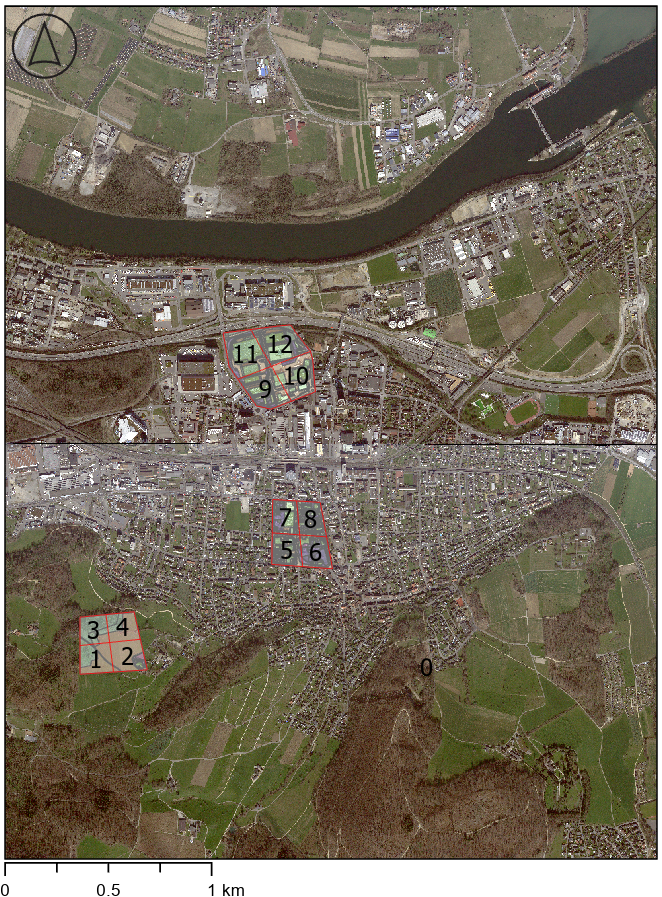
\includegraphics[scale=0.6]{figures/AOI_Labeled.png}
    \caption{The area of interest with the three labeled areas.}
    \label{fig:aoi_labeled}
\end{figure}

\begin{figure}[H]
    \centering
    \captionsetup{width=0.8\linewidth}
    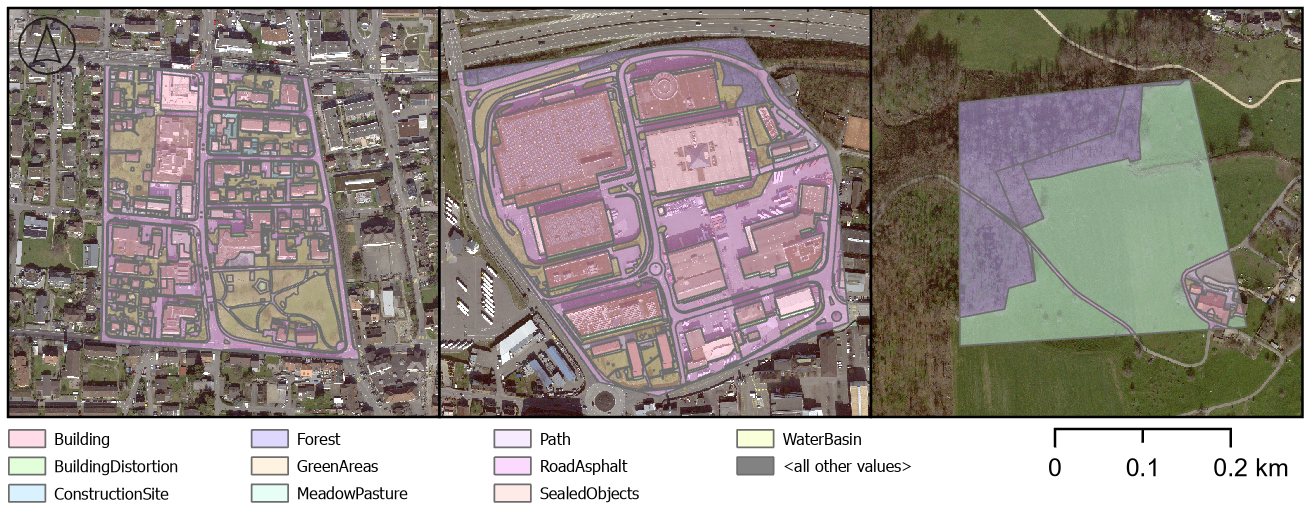
\includegraphics[width=\linewidth]{figures/category_areas.png}
    \caption{The three areas with the corresponding landcover categories.}
    \label{fig:category_areas}
\end{figure}

\autoref{fig:aoi_labeled}
\autoref{fig:category_areas}

\subsection{Data Processing}%%%%%%%%%%%%%%%%%%%%%%%%%%%%%%%%%%%%%%%%%%%%%%%%%%%%

In a first step the data was processed using ArcGIS Pro. The process included a few steps implemented as
a model \autoref{fig:processing_model}.

\begin{figure}
    \centering
    \captionsetup{width=0.8\linewidth}
    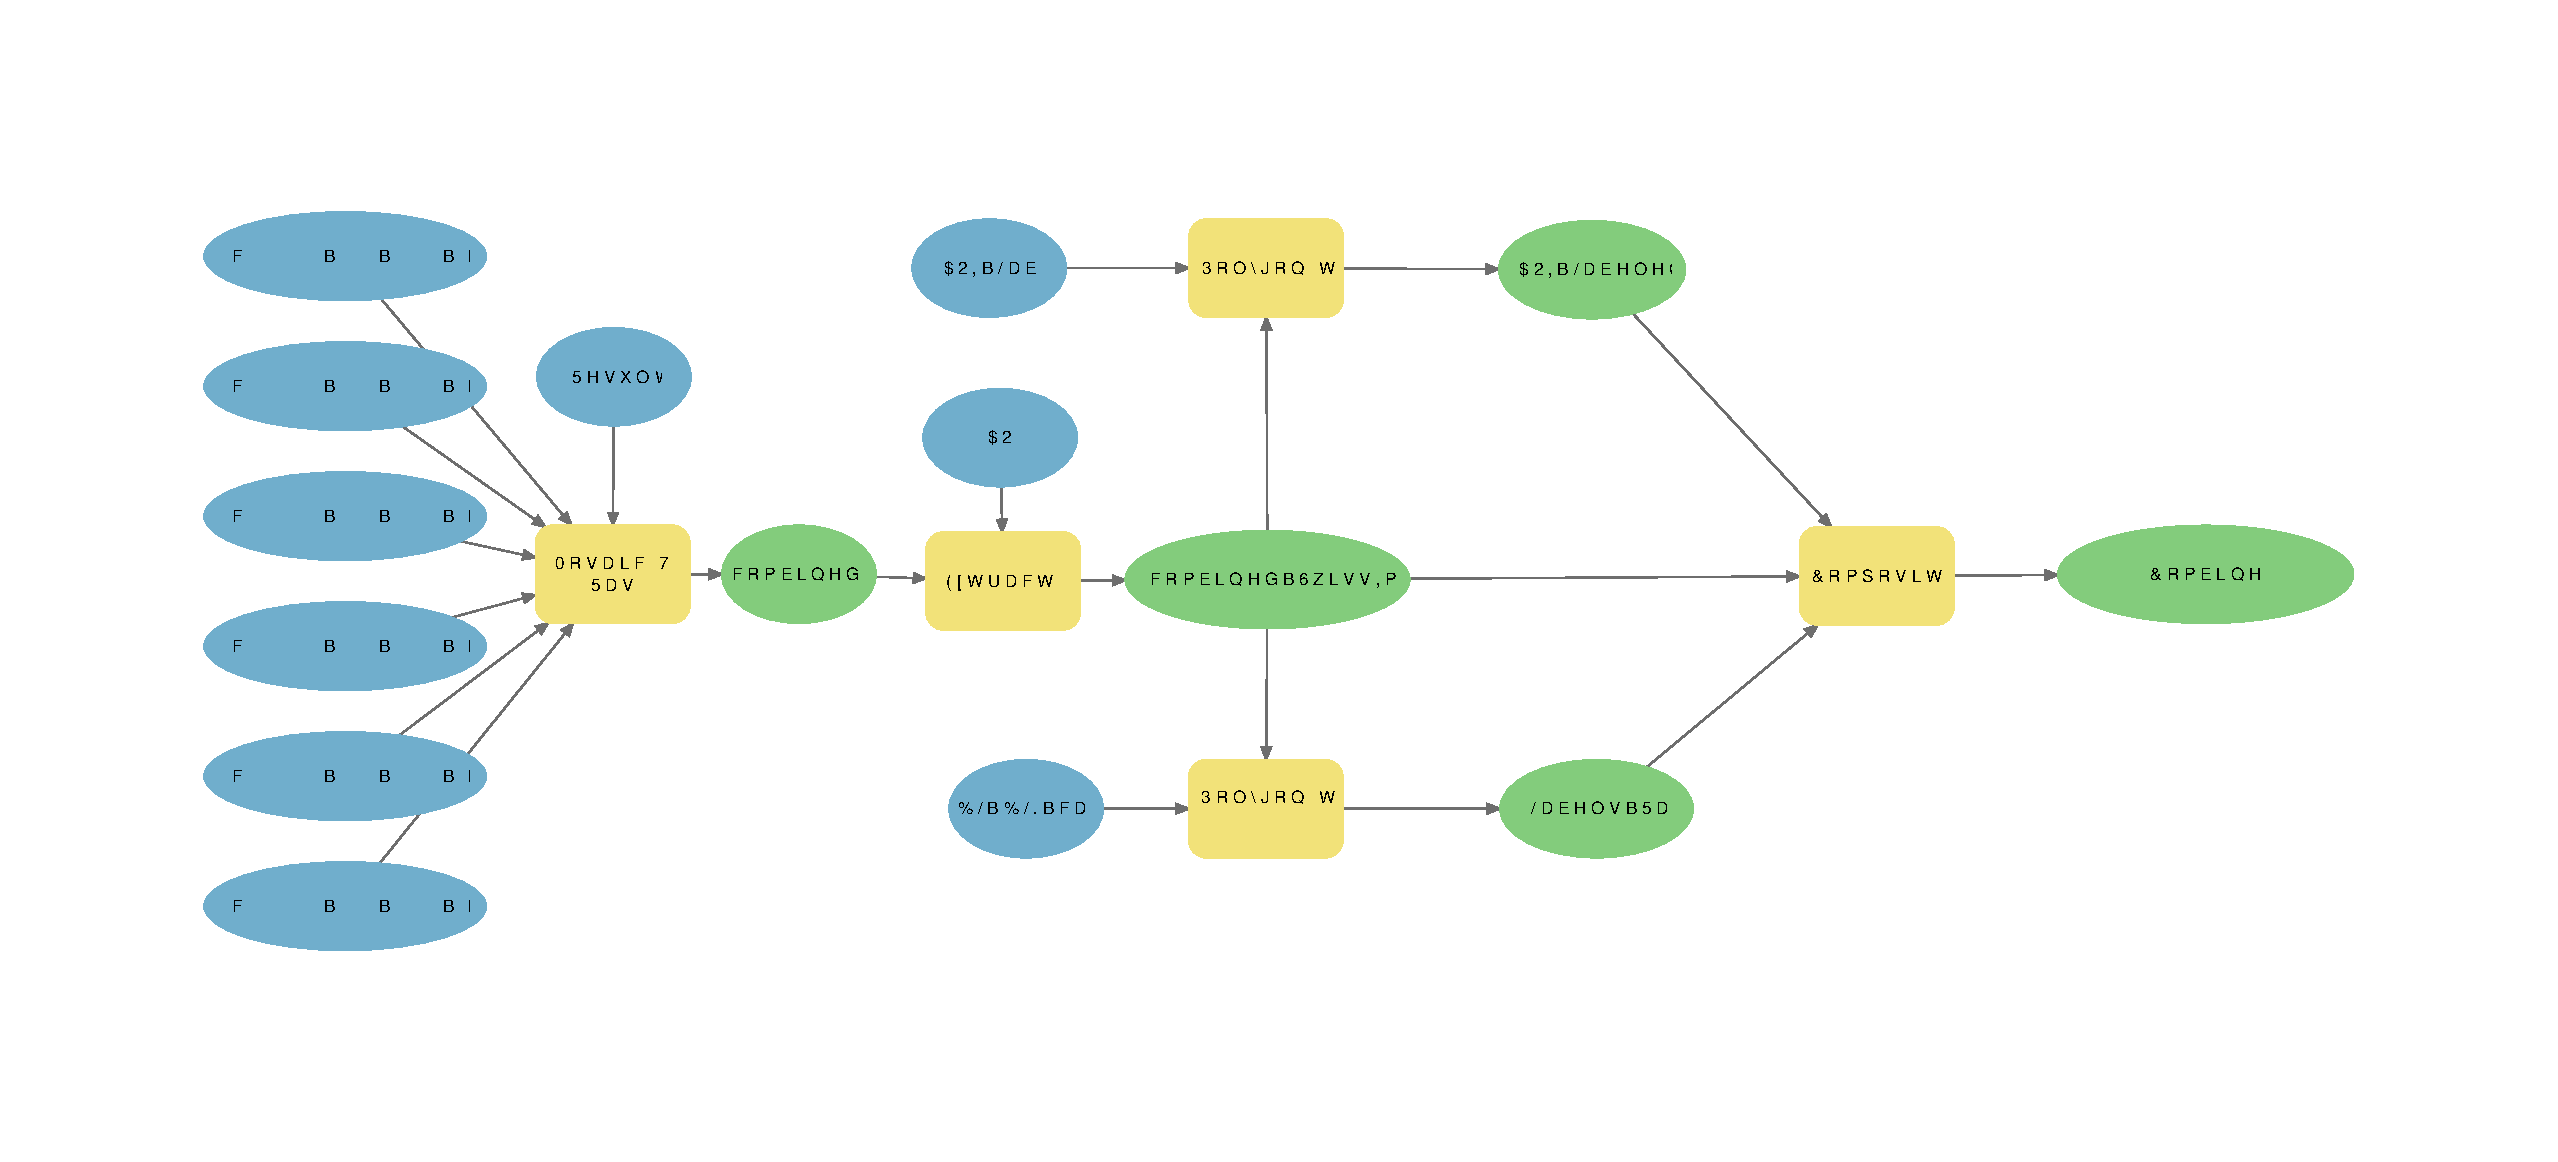
\includegraphics[width=\linewidth]{figures/Model.pdf}
    \caption{The ArcGis model used for preprocessing the data.}
    \label{fig:processing_model}
\end{figure}
% Indicate the main file. Must go at the beginning of the file.
% !TEX root = ../main.tex

%%%%%%%%%%%%%%%%%%%%%%%%%%%%%%%%%%%%%%%%%%%%%%%%%%%%%%%%%%%%%%%%%%%%%%%%%%%%%%%%
% 03_results
%%%%%%%%%%%%%%%%%%%%%%%%%%%%%%%%%%%%%%%%%%%%%%%%%%%%%%%%%%%%%%%%%%%%%%%%%%%%%%%%


\section{Results}
\label{results}

\subsection{Different Label Types}%%%%%%%%%%%%%%%%%%%%%%%%%%%%%%%%%%%%%%%%%%%%%%


\subsection{Augmentation}%%%%%%%%%%%%%%%%%%%%%%%%%%%%%%%%%%%%%%%%%%%%%%%%%%%%%%%


\subsection{Hyperparameter Tuning}%%%%%%%%%%%%%%%%%%%%%%%%%%%%%%%%%%%%%%%%%%%%%%

\begin{figure}[H]
    \centering
    \captionsetup{width=0.8\linewidth}
    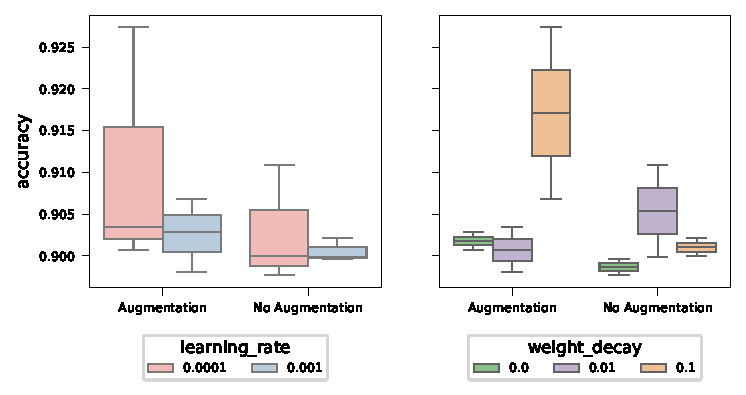
\includegraphics{figures/hp_tuning_boxplot.pdf}
    \caption{Accuracy of the models for the different hyperparameter grouped by use of data augmentation.}
    \label{fig:hp_tuning_boxplot}
\end{figure}



\subsection{Best Model}%%%%%%%%%%%%%%%%%%%%%%%%%%%%%%%%%%%%%%%%%%%%%%%%%%%%%%%%%

The best performing model was the one for the simplified perviousness classification
with the following hyperparameter:
\begin{itemize}
    \item Learning rate: 0.001
    \item Weight decay: 0.01
    \item Data augmentation applied
\end{itemize}
It achieved an accuracy of 0.927 and a weighted F1 Score of 0.927.
The F1 Score per class was 0.92 for class 'unsealed' and 0.93 for class 'sealed'.
The accuracy per category is shown in \autoref{fig:best_model_accuracy_per_category}.
For a visual inspection of the predictions refer to \autoref{fig:best_model_visual}.

\begin{figure}[H]
    \centering
    \captionsetup{width=0.8\linewidth}
    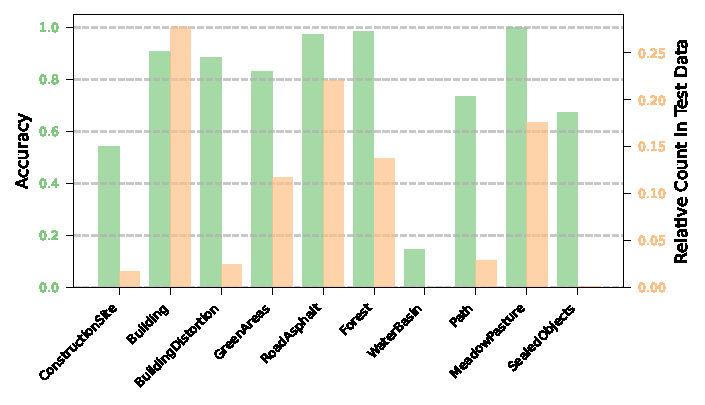
\includegraphics{figures/best_model_accuracy_per_category.pdf}
    \caption{Accuracy per category for the best performing model including relative count of available data for each category.}
    \label{fig:best_model_accuracy_per_category}
\end{figure}

\begin{figure}[H]
    \centering
    \captionsetup{width=0.8\linewidth}
    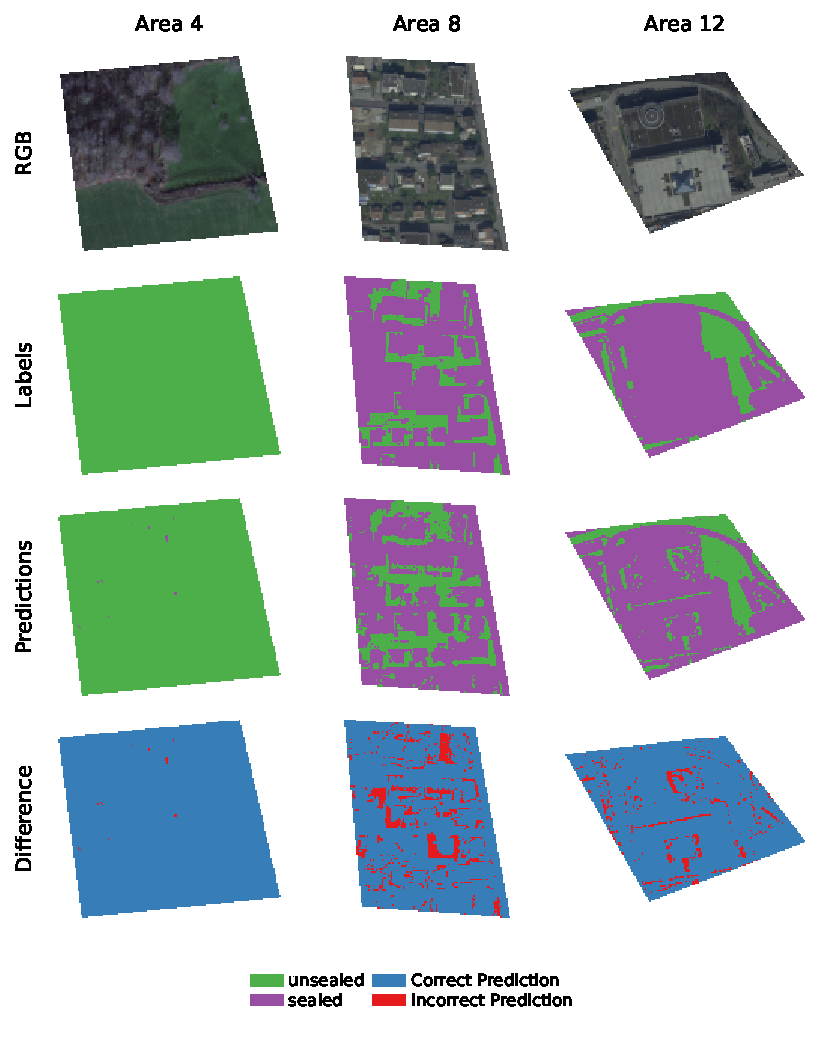
\includegraphics{figures/best_model_visual.pdf}
    \caption{Visual inspection of the predictions for the test areas of the best model.}
    \label{fig:best_model_visual}
\end{figure}
% Indicate the main file. Must go at the beginning of the file.
% !TEX root = ../main.tex

%%%%%%%%%%%%%%%%%%%%%%%%%%%%%%%%%%%%%%%%%%%%%%%%%%%%%%%%%%%%%%%%%%%%%%%%%%%%%%%%
% 04_discussion
%%%%%%%%%%%%%%%%%%%%%%%%%%%%%%%%%%%%%%%%%%%%%%%%%%%%%%%%%%%%%%%%%%%%%%%%%%%%%%%%


\section{Discussion}
\label{discussion}

\subsection{Hyperparameter Tuning}

The hyperparameter tuning process was successful in finding the best hyperparameters
within the grid search. From \autoref{fig:hp_tuning_boxplot}, it can be seen that
lower values for the \texttt{learning\_rate} seem to work better and that
a higher regularization during training -- a higher value of \texttt{weight\_decay} -- leads to
better results. Very interesting is the fact that the benefit of the data augmentation
seems to correlate with more regularization during training.
The grid of evaluated hyperparameters was rather limited due to limited computational
resources and the remaining time. A more extensive search could potentially lead to
even better results. What might really be worth trying is testing even smaller
values of \texttt{learning\_rate}, higher values for \texttt{weight\_decay}, 
and using other options for data augmentation --
pixel- and channel-noise in different combinations.

\subsection{Best Model Performance}

The best-performing model achieved a reasonably high accuracy of 0.92. The validation
metrics, loss, and accuracy, shown in \autoref{fig:best_model_training_metrics},
suggest reasonable progress during the fitting process. Since they both are not
completely flattening out, it might even be possible to further improve the model
using the same architecture and hyperparameters by training it for more epochs.
This could be achieved by using a higher value for the \texttt{patience} parameter --
the next value to be tested could be 20 instead of 10.

\begin{figure}[H]
    \centering
    \captionsetup{width=0.8\linewidth}
    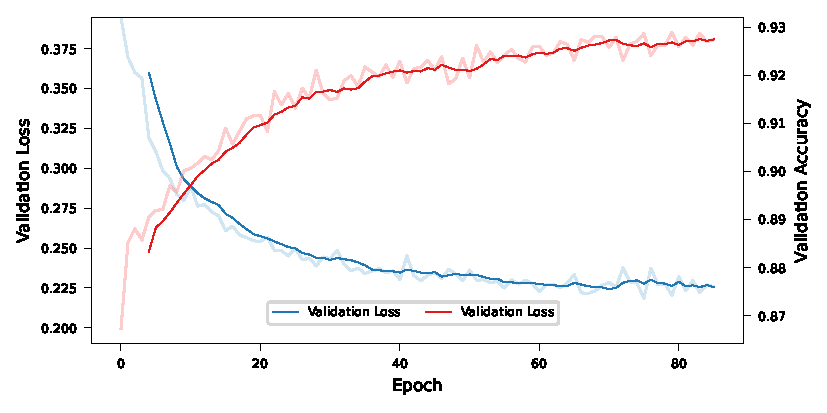
\includegraphics{figures/best_model_training_metrics.pdf}
    \caption{Validation loss and accuracy for the best model.}
    \label{fig:best_model_training_metrics}
\end{figure}

The accuracy per class, shown in \autoref{fig:best_model_accuracy_per_category},
aligns with expectations. Classes like \texttt{Building}, \texttt{GreenAreas}, \texttt{RoadAsphalt}, \texttt{Forest},
and \texttt{MeadowPasture} are predicted with high accuracy. Conversely, classes where there is
very little data available, like \texttt{WaterBasin}, or classes where the data is more vague,
like \texttt{ConstructionSites}, are predicted with lower accuracy.

From the visual inspection of the predictions in \autoref{fig:best_model_visual},  
it looks like the borders between the classes are difficult to predict. This can be  
explained by the fact that the classes are not always very precise, which specifically  
affects these areas. Another explanation could be the resolution of 10 cm,  
which leads to pixels in reality consisting of multiple classes. This issue, referred to  
as mixed pixels, could be part of the reason for the lower accuracy in the  
border areas. This is also supported by \autoref{fig:incorrect_per_category},  
which shows that the incorrectly predicted pixels are often located at the borders  
of objects. Another reason for wrong predictions seems to be inaccuracy in the  
ground truth data. This is especially visible in Area 8 -- the building on the  
top right -- which seems to include some green areas within the building perimeter according to the labels.  
There the model predictions might be more accurate than the ground truth data.  
Another issue seems to be with the \texttt{ConstructionSite} class, where some
areas marked as wrongly predicted might actually be correctly predicted by the model
and incorrectly labeled in the ground truth data. In order to improve the result, a thorough
inspection of the ground truth data might be necessary.

\subsection{Comparing the Results to the GIS Approach}

Since the validation for the original studies was done for a different area in Rünenberg,
using a different dataset, it is hard to compare the results directly. Adding to that,
different land cover categories were used, as well as different resolutions. Overall, the
original studies achieved an accuracy of 0.9 to 1 for the more obvious classes like
\texttt{Buildings}, \texttt{SealedRoads}, \texttt{GreenAreas}, and \texttt{MeadowPastures}. 
For the more difficult classes, like \texttt{PathUnsealed} and \texttt{SealedObjects}, the
accuracy was lower as well. The results of this study -- as differently as they were created --
reach a similar range of accuracy.

\subsection{Prospects}

The results of this study show that the approach of using deep learning for perviousness
classification is promising. The results are in a similar range as the results of the
original study using a GIS approach. Therefore, it might be worth further investigating
the potential of deep learning for this task. The next steps, besides the mentioned hyperparameter
expansion, more data augmentation, and more thorough training by going for more epochs, include other
promising approaches. One could be to try different model concepts like U-Net -- specifically
designed for image segmentation tasks. Another approach could be to use a pre-trained model
to build upon -- the issue there is finding a model that is trained on similar data and
accepts four channels as input. Another idea could be to implement some self-supervised
learning techniques utilizing unlabeled data to improve the model. As with most deep
learning tasks, the more data, the better -- so it would be worth trying to get more data
of possibly even higher quality to improve the existing models.

% Indicate the main file. Must go at the beginning of the file.
% !TEX root = ../main.tex

%%%%%%%%%%%%%%%%%%%%%%%%%%%%%%%%%%%%%%%%%%%%%%%%%%%%%%%%%%%%%%%%%%%%%%%%%%%%%%%%
% 05_acknowledgment_declaration
%%%%%%%%%%%%%%%%%%%%%%%%%%%%%%%%%%%%%%%%%%%%%%%%%%%%%%%%%%%%%%%%%%%%%%%%%%%%%%%%


\section{Acknowledgment and Declaration}
\label{acknowledgment_declaration}

\subsection{Acknowledgment}%%%%%%%%%%%%%%%%%%%%%%%%%%%%%%%%%%%%%%%%%%%%%%%%%%%%%%

I thank Dr. Johann Junghardt for his support.
I would like to express my gratitude to my brother, Dr. Basil Kraft, for his continuous
support with his expertise in the field of machine learning. 

\subsection{Declaration of AI Usage}%%%%%%%%%%%%%%%%%%%%%%%%%%%%%%%%%%%%%%%%%%%%%%

GitHub Copilot was used to assist writing the code and text for this project.

ChatGPT was used to assist researching as well as writing the code and text for this project.

Sections of the text generated by ChatGPT 4o revised by the author are:
\begin{itemize}
    \item Abstract
    \item Introduction
    \item Model Architecture
\end{itemize}

\newpage
\refstepcounter{subsection}
\addcontentsline{toc}{subsection}{\protect\numberline{\thesubsection}Statement of Authorship}

\newgeometry{left=0in, right=0in, top=0.5in, bottom=0in}
\thispagestyle{empty}
\begin{figure}[h!]
    \centering
    
\includegraphics[width=0.9\textwidth]{figures/declaration_independence.pdf}
\end{figure}
\restoregeometry % Restore original margins


\printbibliography[heading=bibintoc]

\appendix
% \include{sections/a_tables}

\end{document}  
